
\label{chap:experimental_results}

This chapter discusses a number of experimental results obtained using the implemented PDP firmware discussed in Chapter~\ref{chap:implementation}. Only select results are included. These were chosen because they provide direct evidence that the protocol and PDP firmware solve the challenges put forth in Chapter~\ref{chap:problem_formulation} and meet the design goals discussed in Chapter~\ref{sec:design_methodology}.

 Firstly, memory synchronizer operation is discussed and evaluated because correct clock domain crossing is an essential requirement for array operation. Secondly, overall firmware behavior is evaluated in both simulation and practice. Thirdly, packetized operation is evaluated. Finally, overall results are discussed to provide a summary of lessons learned during operational testing.

\section{Memory Synchronizer}

    This section describes the various tests performed on the full/empty memory synchronizer used within the PDP firmware to synchronize data transitioning across clock domains. First, it discusses simulation results obtained through a full behavioral simulation of the PDP firmware. Secondly, it discusses using the memory synchronizer in a test setup and the pitfalls that occurred with earlier implementations.

    \subsection{Simulation}
        Figure~\ref{fig:full_empty_sim} shows the simulated results of the full/empty memory synchronizer when transitioning to full and back to empty for a writer and reader operating at \mbox{35.75 megahertz} and \mbox{200 megahertz}, respectively. For discussion about each signal and expected internal behavior see Chapter~\ref{sec:memorysync}. Each state transition in the simulation should look similar to the state transitions shown in Table~\ref{tbl:full_empty_circuit_states}.

        \begin{figure}[t]
            \centering
            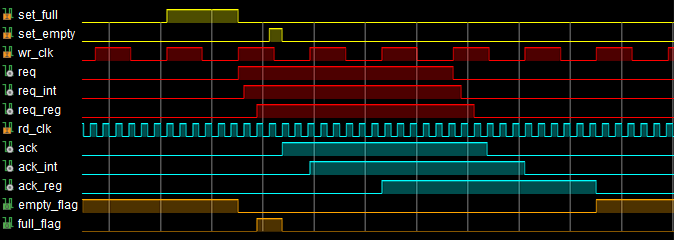
\includegraphics[width=1.0\textwidth]{fig/full_empty_sim.png}
             \caption{Behavioral Simulation of a Single Pixel Being Buffered Through the Full/Empty Memory Synchronizer}
            \label{fig:full_empty_sim}
        \end{figure}

        The circuit holds a steady state until the {\it set full} signal is toggled for a single {\it write clock} cycle. On the next {\it write clock} cycle, the {\it req signal} transitions high and the {\it empty flag} transitions low. Then the data is moved to the {\it read clock} domain using the two flip-flop synchronizer scheme discussed in the implementation details. At the next rising edge of the {\it read clock}, the data is latched into {\it req internal} which is an internal metastable register. Due to the speed difference between write and read clock speed, the data latches into the register quickly. Following this, a cycle later, the data is clocked into {\it req reg} which completes the {\it read clock} domain transition causing the {\it full flag} to transition high.

        Once any corresponding buffer data is handled by the PDP firmware, the {\it set empty} signal is toggled for a single {\it read clock} cycle. This causes the {\it ack} signal to transition high. Then the data is moved to the {\it write clock} domain using the two flip-flop synchronizer scheme discussed in the implementation details. At the next rising edge of the {\it write clock}, the data is latched into {\it ack internal}. Following this, a cycle later, the data is clocked into {\it ack reg} which completes the {\it write clock} domain transition. Notice that it takes much longer to transition data from the {\it read clock} domain to the {\it write clock} domain than vice versa. This is due to the slow write clock.

        A {\it write clock} cycle later, {\it req} transitions low. Subsequently, it transitions to the {\it read clock} domain just as before. Following this, the {\it ack} line is lowered and transitions to the {\it write clock} domain just as before. At the same time, the {\it empty flag} transitions high, and the circuit is in the state it began in.

        This follows the expected state transitions from Table~\ref{tbl:full_empty_circuit_states} with the only notable distinction being that transitions across clock domains take different amounts of time depending on the sources clock speed.

        In practice, a complete double handshake takes many cycles to complete which could lead to undesired overflow behavior. In PDP, overflow issues are mitigated by allocating enough internal buffers to allow for there to always be a buffer available for a writer to fill.

        Additionally, the use of the two flip-flop synchronizer means that it takes more than a single {\it read clock} cycle for the {\it full flag} to raise; however, given that the pixels of an IRLED array take many {\it read clock} cycles to charge, this does not pose a problem. Moreover, in practice, the {\it full flag} transitions in between two to three cycles of the reader clock depending on where the rising edge of the reader clock falls relative to the transitioning of the {\it req} signal.

        Figure~\ref{fig:full_empty_row_sim} shows the simulated results of the full/empty memory synchronizer with multiple pixels being buffered through it for a writer and reader operating at \mbox{35.75 megahertz} and \mbox{200 megahertz}, respectively. The large gaps of time between transitions to full are due to there being multiple buffers available as discussed above. This indicates that at the simulated rates no overflow is occurring. In practice, it would be possible for overflow to occur if the write clock speed were close to the read clock speed; however, due to the maximum possible write speed for HDMI only being \mbox{148.5 megahertz} and the fact that clock domain crossing latency is hidden through the usage of multiple buffers, a \mbox{200 megahertz} input clock is sufficient for correct behavior.

        \begin{figure}[t]
            \centering
            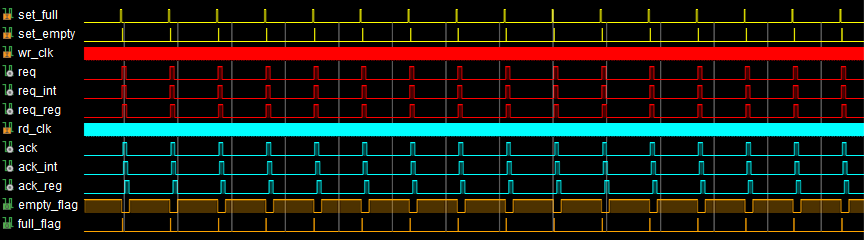
\includegraphics[width=1.0\textwidth]{fig/full_empty_row_sim.png}
            \caption{Behavioral Simulation of Multiple Pixels Being Buffered Through the Full/Empty Memory Synchronizer}
            \label{fig:full_empty_row_sim}
        \end{figure}

    \subsection{Experimental Testing}
        \label{sec:experimental_testing}
        Testing the memory synchronizer on real hardware was an important consideration because behavioral simulations do not capture timing behavior accurately. In real hardware, noise, clock jitter, and variations in synthesis introduce unpredictability that can lead designs to fail unexpectedly if they have inherent metastability issues.

        Testing was performed using a ZYBO development board~\cite{Digilent2016} hooked up as shown in Figure~\ref{fig:zybo_setup}. Image data consisting of 256 by 256 pixels operating at \mbox{250 hertz} was sent over from a test PC to a ZYBO board running an implementation of the synchronized circular buffer. VGA was used to provide loop-back for visual inspection. It is not possible to check for bit-level accuracy using a VGA device due to the analog nature of the interface so a UART device was used as an alternative (slow) path to read out internal image data. It was also used to collect statistical information such as the error bits for a given configuration and the amount of data that passed through the interface.

        \begin{figure}[t]
            \centering
            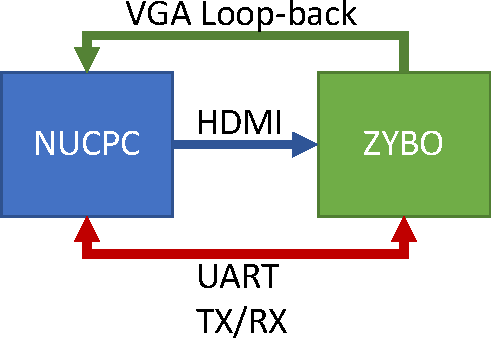
\includegraphics[width=0.40\textwidth]{fig/zybo_setup.pdf}
            \caption{ZYBO Test Setup}
            \label{fig:zybo_setup}
        \end{figure}

        For the first test, the synchronized circular buffer circuit was driven using the checkerboard input image shown in Figure~\ref{fig:checker_pattern}. This pattern was routed to the loop-back device for visual inspection. It was manually retrieved over UART and diffed with the original image to check for bit-level accuracy.

        \begin{figure}[t]
            \centering
            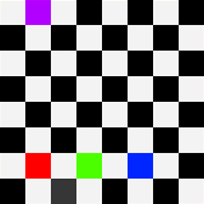
\includegraphics{fig/checker.png}
            \caption{Checkerboard Input Image}
            \label{fig:checker_pattern}
        \end{figure}

        For the second test, a dynamic CRC-like pattern was used to verify data accuracy directly. Segments of eight 8-bit random values where generated and then inserted into an HDMI stream twice as shown in Figure~\ref{fig:crc_like_buffer}. The pattern dynamic changed for every input frame. Figure~\ref{fig:random_noise} shows an example pattern. Internally, the test circuit would compare the results of the segments and log errors. UART was used to retrieve the error count.

        \begin{figure}[t]
            \centering
            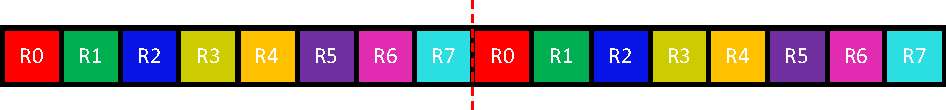
\includegraphics[width=0.75\textwidth]{fig/crc_like_buffer.pdf}
            \caption{CRC-like 16-pixel Stream}
            \label{fig:crc_like_buffer}
        \end{figure}

        \begin{figure}[t]
            \centering
            
\includegraphics{fig/random_noise.png}
            \caption{CRC-like Input Image}
            \label{fig:random_noise}
        \end{figure}

        The initial synchronizer circuit employed within the design was able to pass behavioral simulation but during the experimental testing phase exhibited bit-level errors. Upon careful analysis, it was discovered that the design contained metastability issues due to how the synthesizer routes signals during synthesis. The early design employed a clock switching strategy within the memory synchronizer circuit. Essentially, the clock of the circuit was switched depending on whether the circuit was full or empty. In practice, this would randomly result in bit corruption depending on how the circuit synthesized due to variability in the routing process. As a consequence, the timing delays between components would change unpredictably between different synthesized runs and ultimately led to a metastable clock handoff which resulted in the circuit entering an inconsistent state. The final design discussed in this dissertation removes the clock switching circuitry and instead employs the double handshake design discussed in Chapter~\ref{sec:memorysync} in order to guarantee correct operation. The test patterns discussed above were able verify this.

\section{Firmware}
    This section discusses behavioral simulations of the PDP firmware implementation and experimental results obtained from running the firmware on actual IRLED arrays. The simulations serve to verify correct operational logic and the experimental results serve to validate the timing behavior of the implemented circuits.

    \subsection{Simulation}
    This section provides captures of a few simulation inputs and outputs to show how packets arrive and are processed by the PDP firmware architecture. Other isolated module and integrated simulations (not shown here) were performed to access behavioral operation within the PDP firmware circuitry. Additional module level unit testing was performed as well.

    In Figure~\ref{fig:input_example}, simulated HDMI is shown. When video data enable (write enable) transitions high words of data representing PDP packets start to stream in. These are indicated by packet ID, X start, X end, Y start, Y end, and Packet Data. Each word would be stored in an SCB slot as indicated in the previous section. The final piece of data indicated is a reset packet ID.

    \begin{figure}
        \centering
        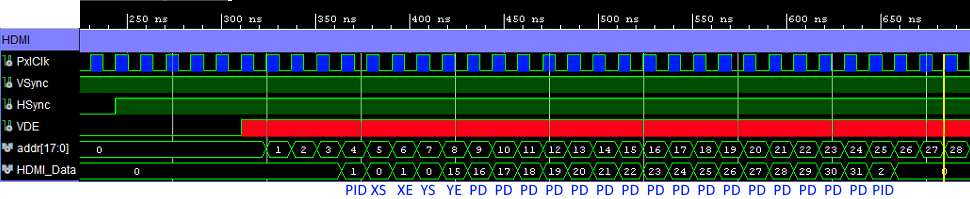
\includegraphics[width=1.0\textwidth]{fig/pdp_input_example.png}
        \caption{Simulation of Single HDMI Input}
        \label{fig:input_example}
    \end{figure}

    Figure~\ref{fig:output_example} shows the final output which would be passed to an array in a real system. Highlighted in red is data from the write enable packet. Note, all values out are up shifted by 5 bits to be received by the DACs in the system. Additionally, the values are shown in reverse order from the input diagram. For example, 992 corresponds to the value of 31 on the input side. In purple the reset packet is shown with two stages of array writes. In the first stage, the load signal transitions to low. In the second stage the load signal transitions high. The states shown are the transitioning stages of the state machines discussed in Chapter~\ref{sec:state_machines}.

    \begin{figure}
        \centering
        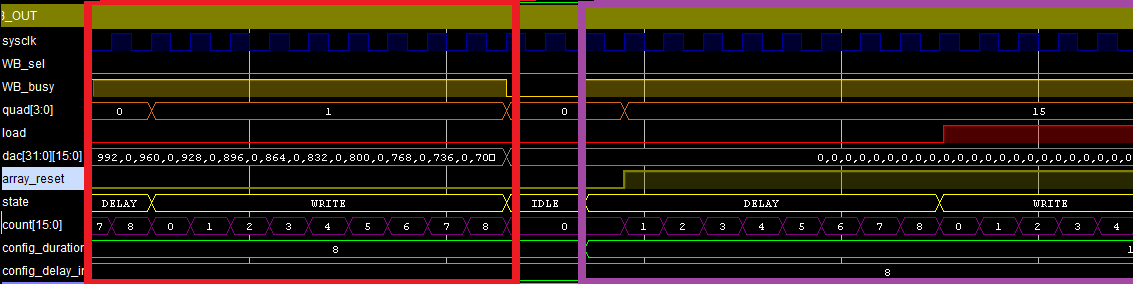
\includegraphics[width=1.0\textwidth]{fig/pdp_output_example.png}
        \caption{Simulation of PDP Output}
        \label{fig:output_example}
    \end{figure}

    \subsection{Characterization}
        This section shows select results of running the PDP firmware on an NSLEDS array to characterize its behavior. Namely, whether it correctly draws to an array and whether it performs better than earlier firmware incarnations. Some non-uniformity corrected imagery is also shown which indicates the PDP firmware is capable of drawing full imagery correctly. Though, only a few results are shown here, the PDP firmware has been run on multiple NSLEDS and HDILED arrays to collect data and characterize the arrays themselves. As of this writing, it has been used in daily operations on my research group's IRLED arrays for over a year and is the primary firmware in use today.

        \subsubsection {Array Maps}
            In order to characterize whether the behavior of the PDP firmware is consistent with older firmware (called SNAP) and has reproducible results between runs, a number of different array characterization tests were performed on an NSLEDS array.

            In one test, an array map is collected which is performed by doing a sweep of array pixels by outputting light to each pixel separately over multiple frames and capturing the result. Typically, this is done using grids to speed up data collection. An example grid for a partial frame is shown in Figure~\ref{fig:grid_sweep}. Defective pixels on an array have low light output or have inconsistent brightness from run to run. This could also happen if a firmware contained internal timing issues as well. Comparing a test firmware with a known good reference firmware can rule out firmware issues in the advent of this type of poor array behavior.

            \begin{figure}[t]
                \centering
                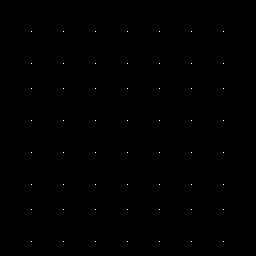
\includegraphics{fig/grid.jpg}
                \caption{Pixel Sweep Grid}
                \label{fig:grid_sweep}
            \end{figure}

            Figure~\ref{fig:array_map_pdp} shows an array map collected from the PDP firmware and Figure~\ref{fig:array_map_snap} shows an array map collected from the older SNAP firmware. In each figure, array data collected using an IR camera is shown on the left with a camera count scale on the right. Camera counts are an uncalibrated measure of IR intensity that can mapped to apparent temperature when calibrated. At a glance, each image appears to be the same; however, the PDP firmware has a slightly higher light output. The dark regions of each map are physically dead pixels on the array. More than half of the particular array is nonfunctioning. The repeating patterns of horizontal lines that can be seen are the result of slow channels on the array. Every 32 columns there are 2 channels which take longer to settle and that can be seen in these results, as these channels have not fully settled. This is due to a design flaw on early arrays which resulted in higher capacitance on those lines. Overall, the PDP firmware results are as expected and indicate correct operation.

            \begin{figure}[t]
                \centering
                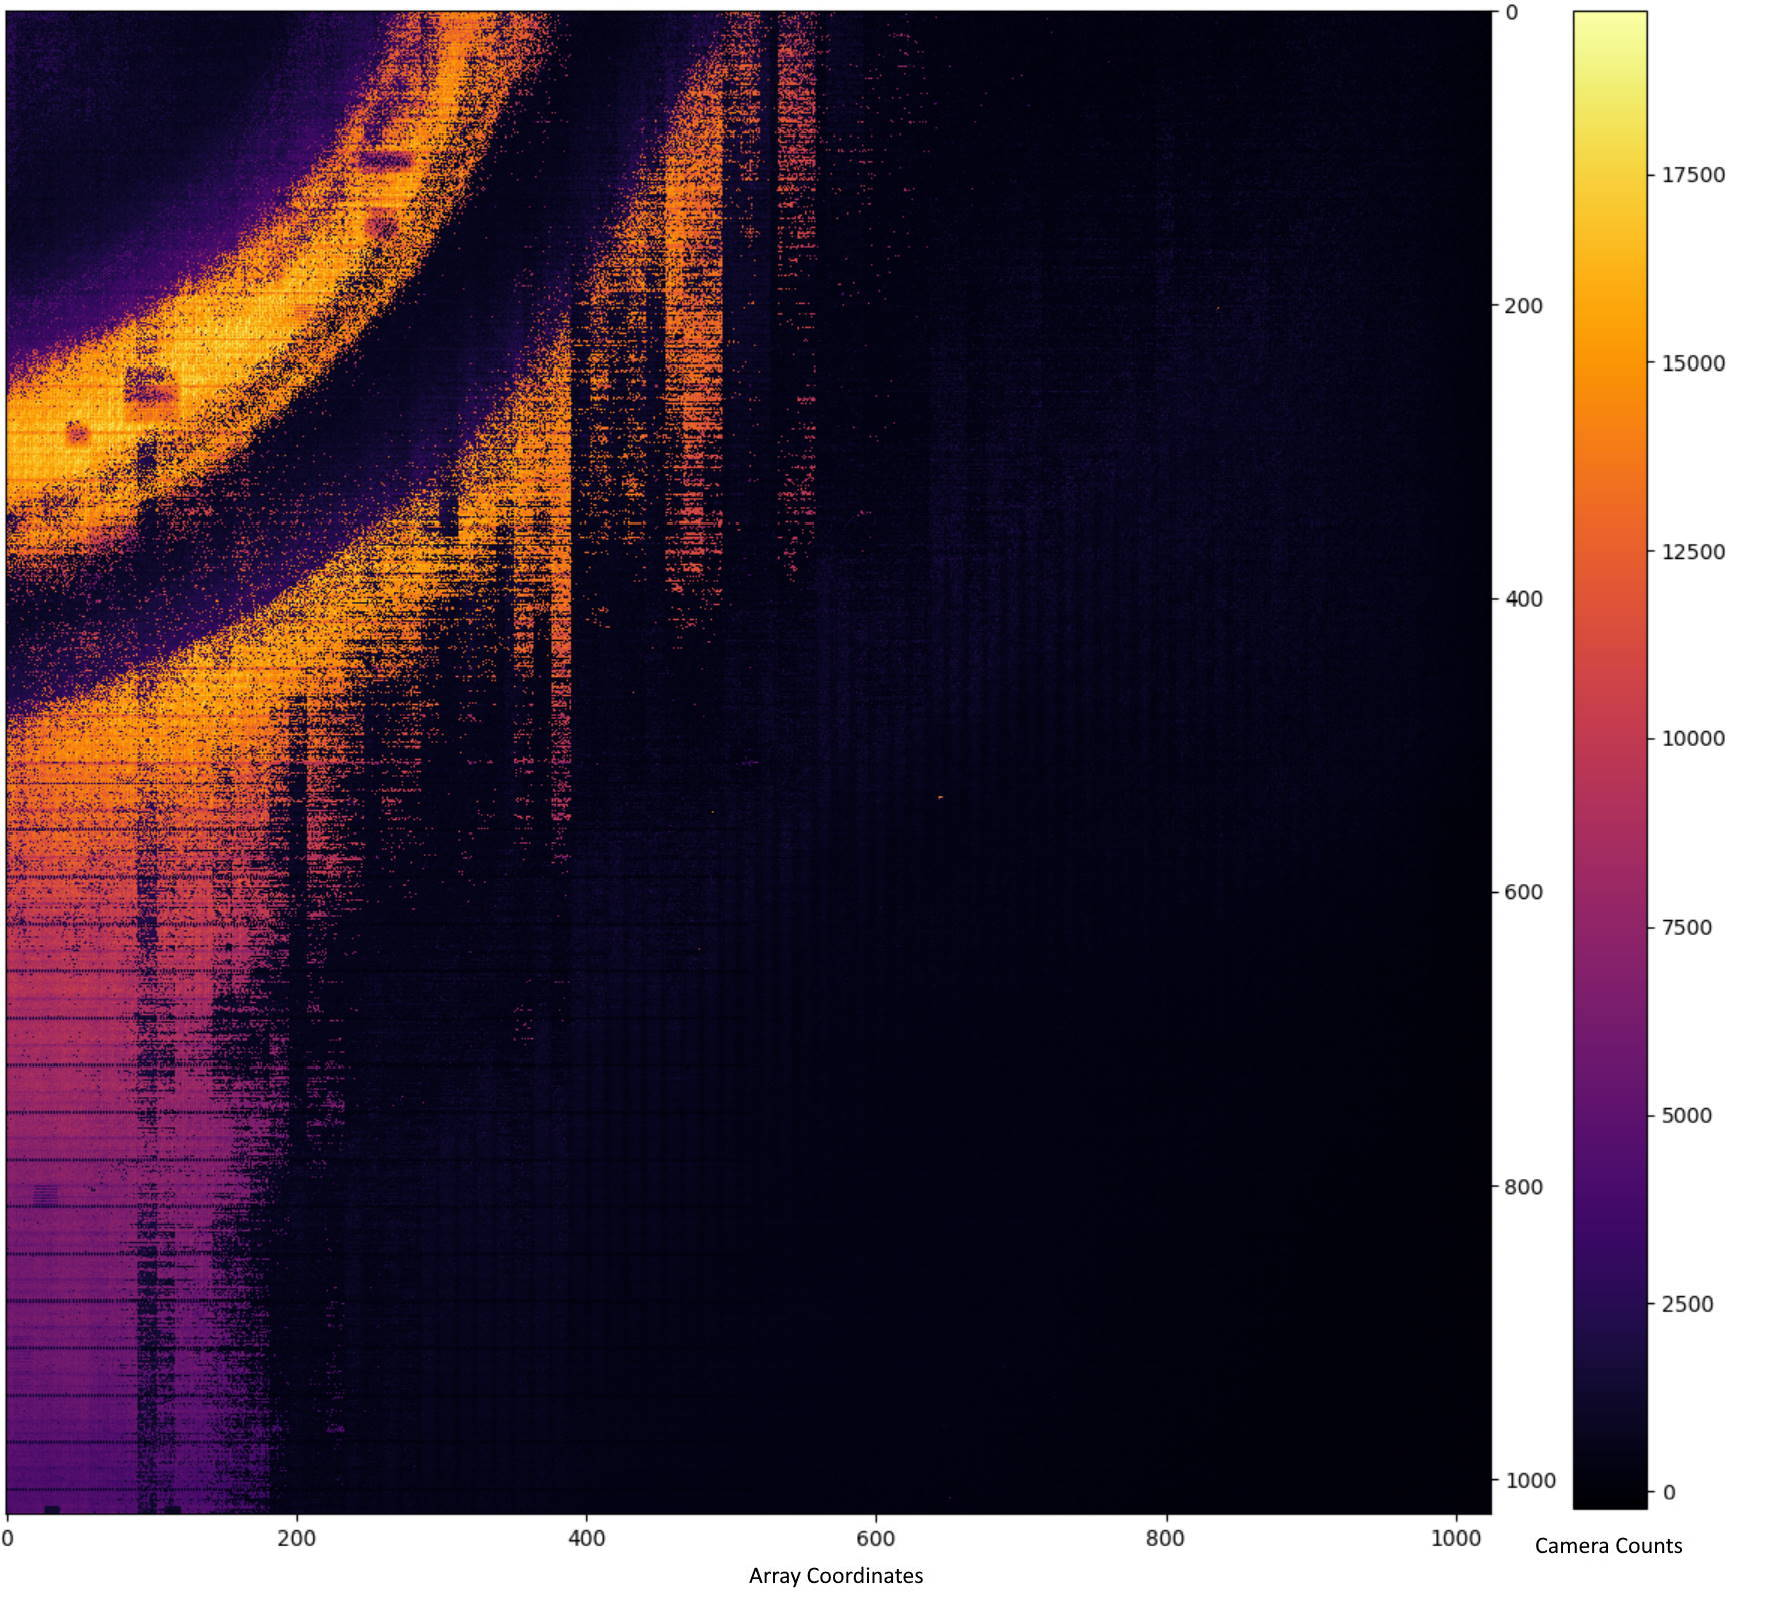
\includegraphics[width=1.0\textwidth]{fig/array_map_pdp.jpg}
                \caption{Array Map of PDP Firmware Output}
                \label{fig:array_map_pdp}
            \end{figure}

            \begin{figure}[t]
                \centering
                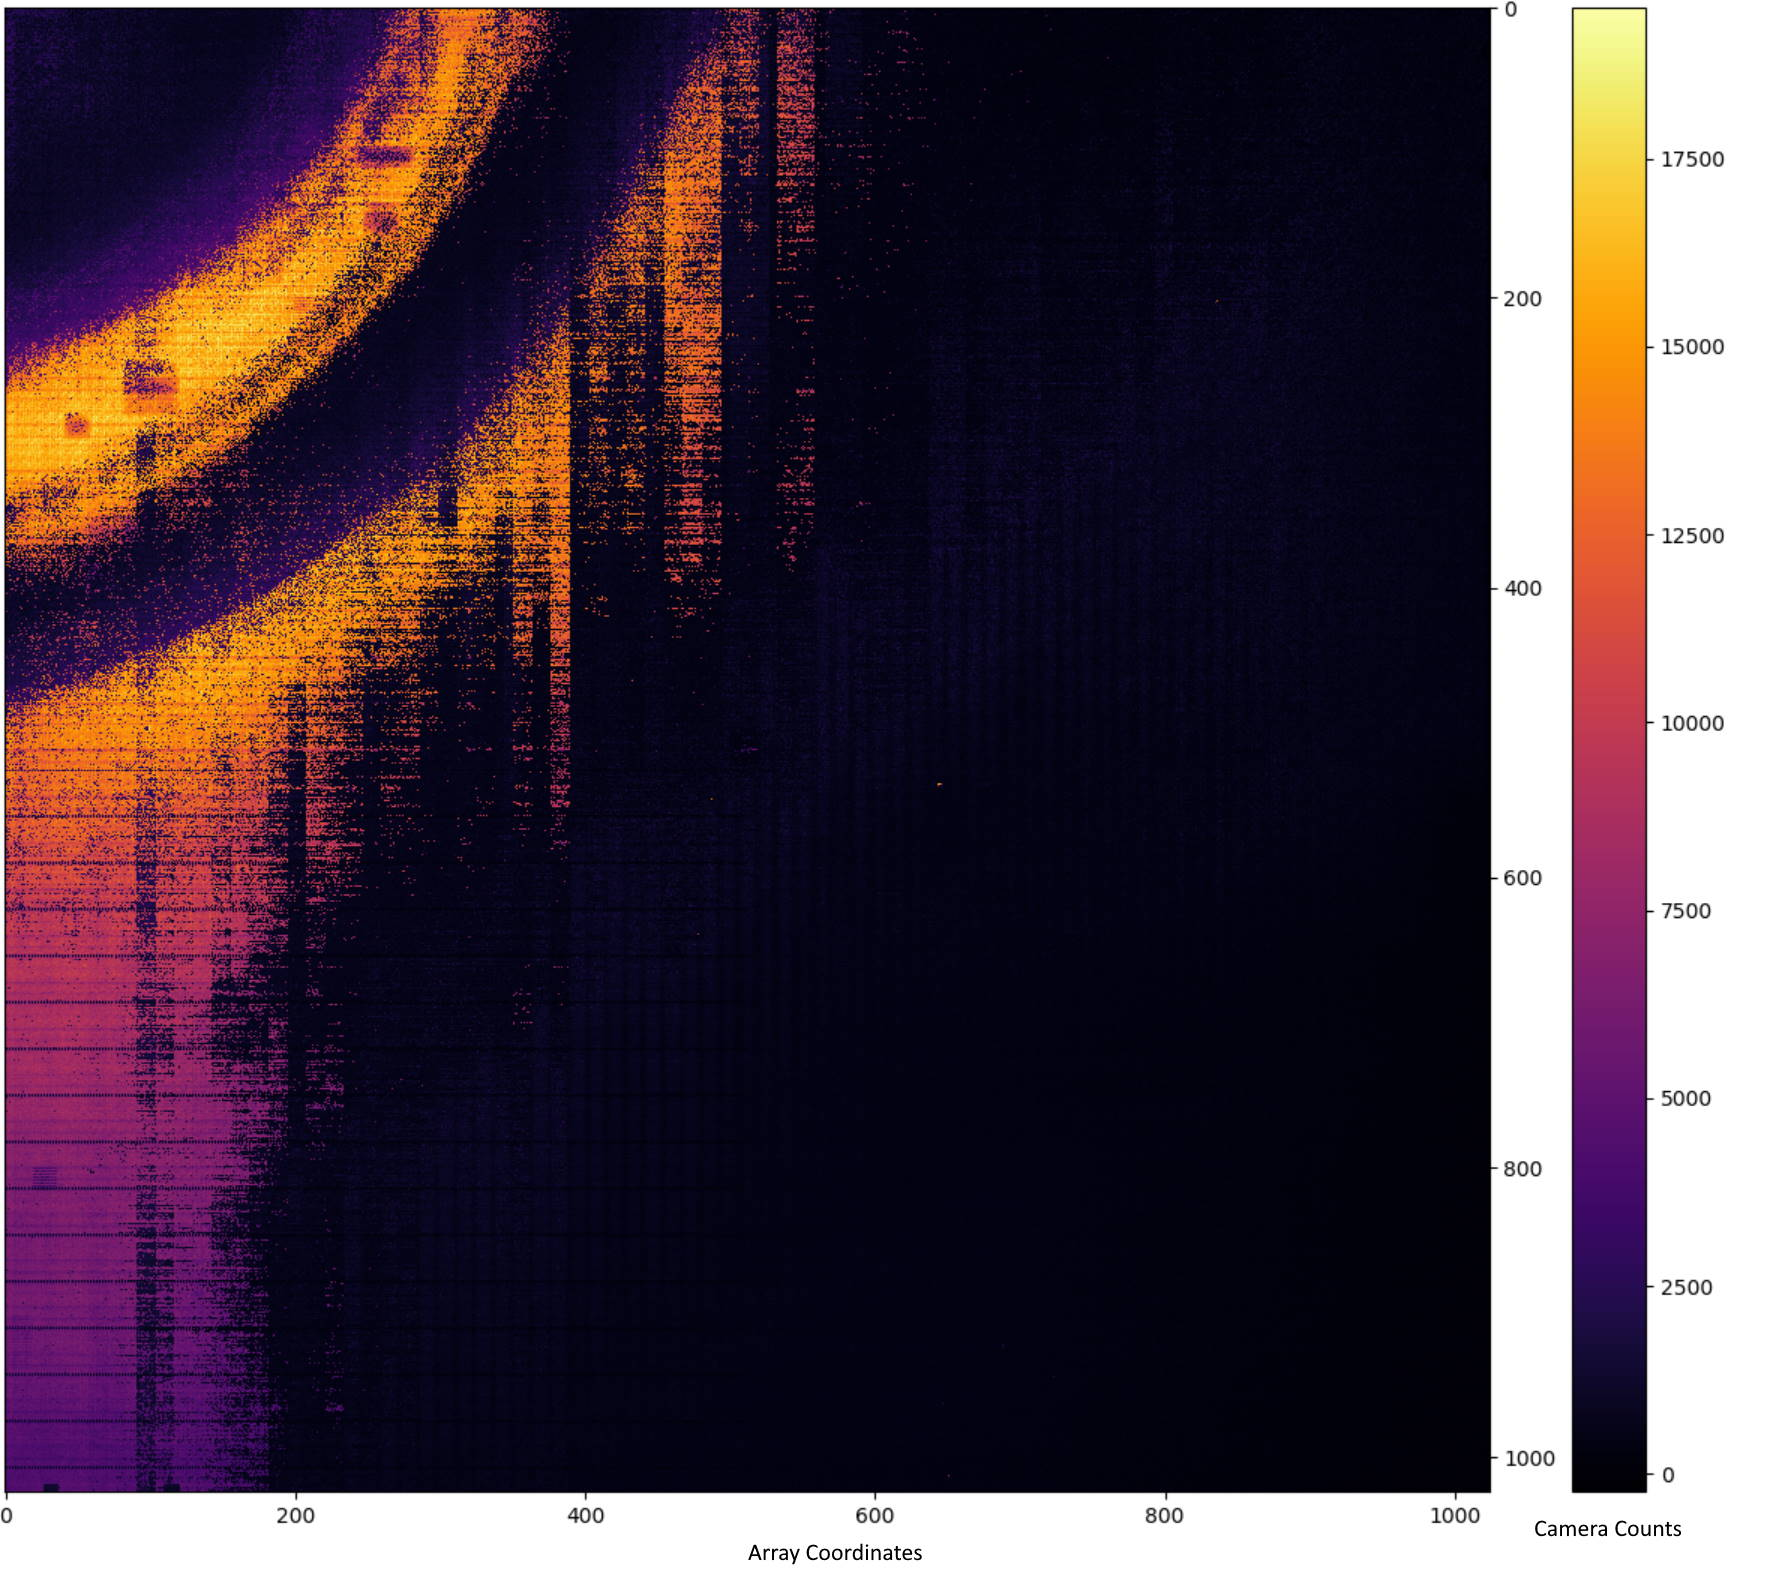
\includegraphics[width=1.0\textwidth]{fig/array_map_snap.jpg}
                \caption{Array Map of SNAP Firmware Output}
                \label{fig:array_map_snap}
            \end{figure}

        \subsubsection{Fractional Difference Maps}

            Another test is to collect multiple array maps and take the fractional difference between them to see the percent difference in light output between runs. This allows for the consistency of light output to be characterized. A large difference could indicate problems with the pixels of an array, analog chain, or firmware behavior. Small differences indicate that the pixels of an array are more consistent between runs. Differences in behavior between firmware (or firmware revisions) would be indicative of variance in signal timing. In this case, a larger variance would indicate less precise timing within the firmware. Some variance is expected is due to camera focus, noise, and physical vibration. The particular IR camera used to collect data in this setup utilizes a motorized reversed-stirling cryo-cooler. These are often utilized for cooling detectors within thermal imaging systems~\cite{Organ1999}. These induce a physical vibration which can result in noise within collected camera imagery.

            Figure~\ref{fig:fractional_difference_pdp} shows a fractional difference map for the PDP firmware and Figure~\ref{fig:fractional_difference_snap} shows a fractional difference map for the older SNAP firmware. The dark blue areas indicating zero difference are dead regions of the array similar to the earlier results. The red areas of high variance are due to those pixels being located on marginal portions of the array specifically along non-functioning edges. In practice for displaying imagery, these areas would be marked as defected and not driven.

            \begin{figure}[t]
                \centering
                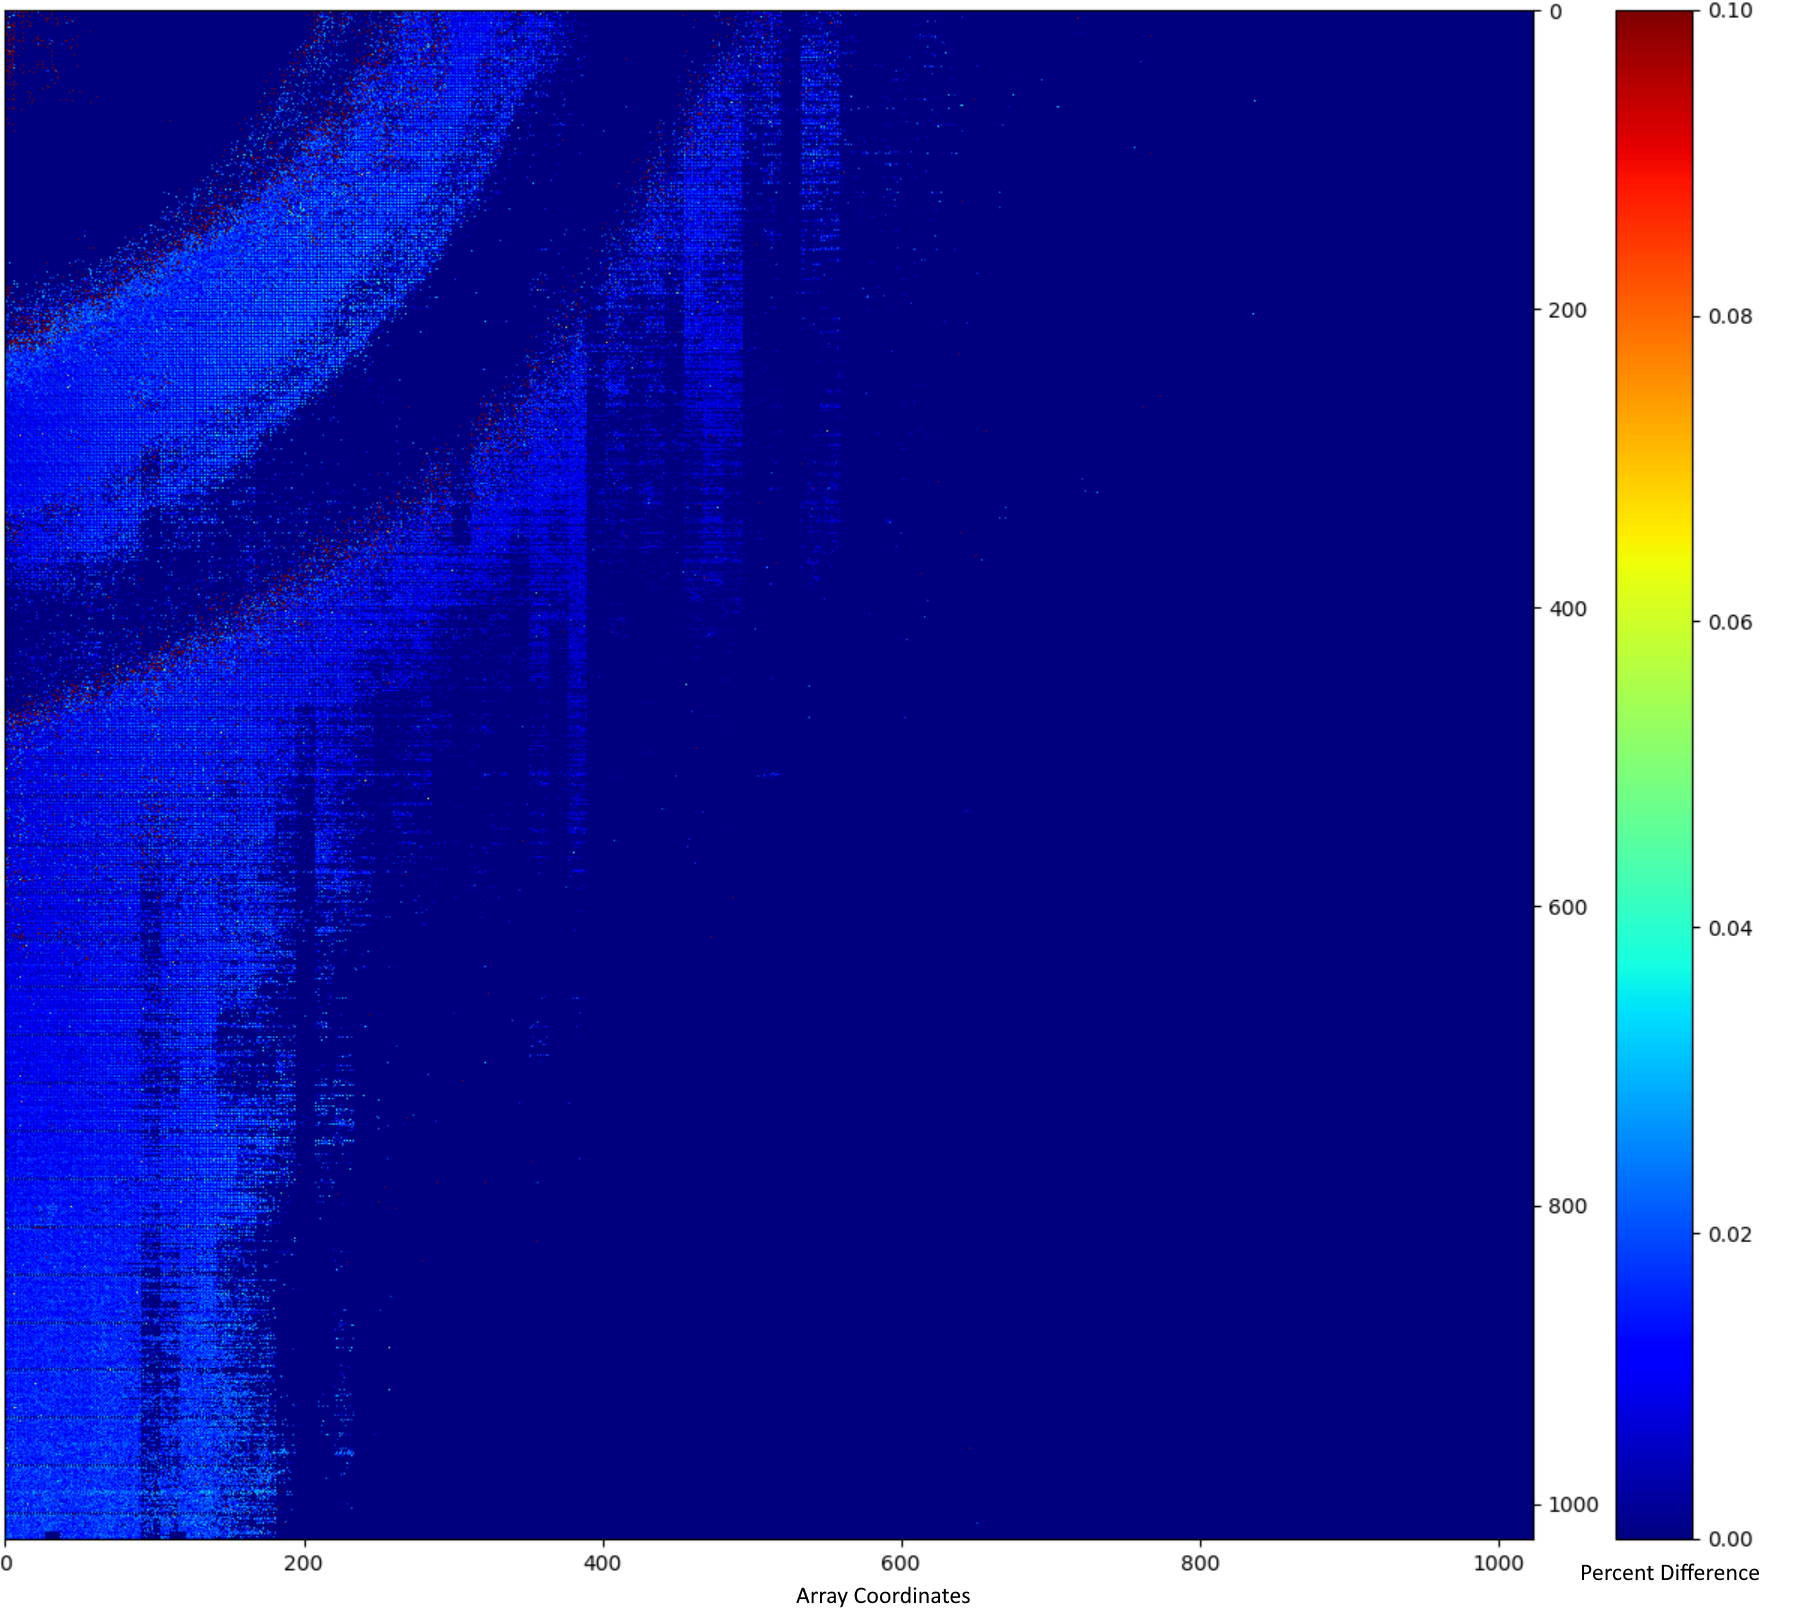
\includegraphics[width=1.0\textwidth]{fig/fractional_difference_pdp.jpg}
                \caption{Fractional Difference Map of PDP Firmware Output}
                \label{fig:fractional_difference_pdp}
            \end{figure}

            \begin{figure}[t]
                \centering
                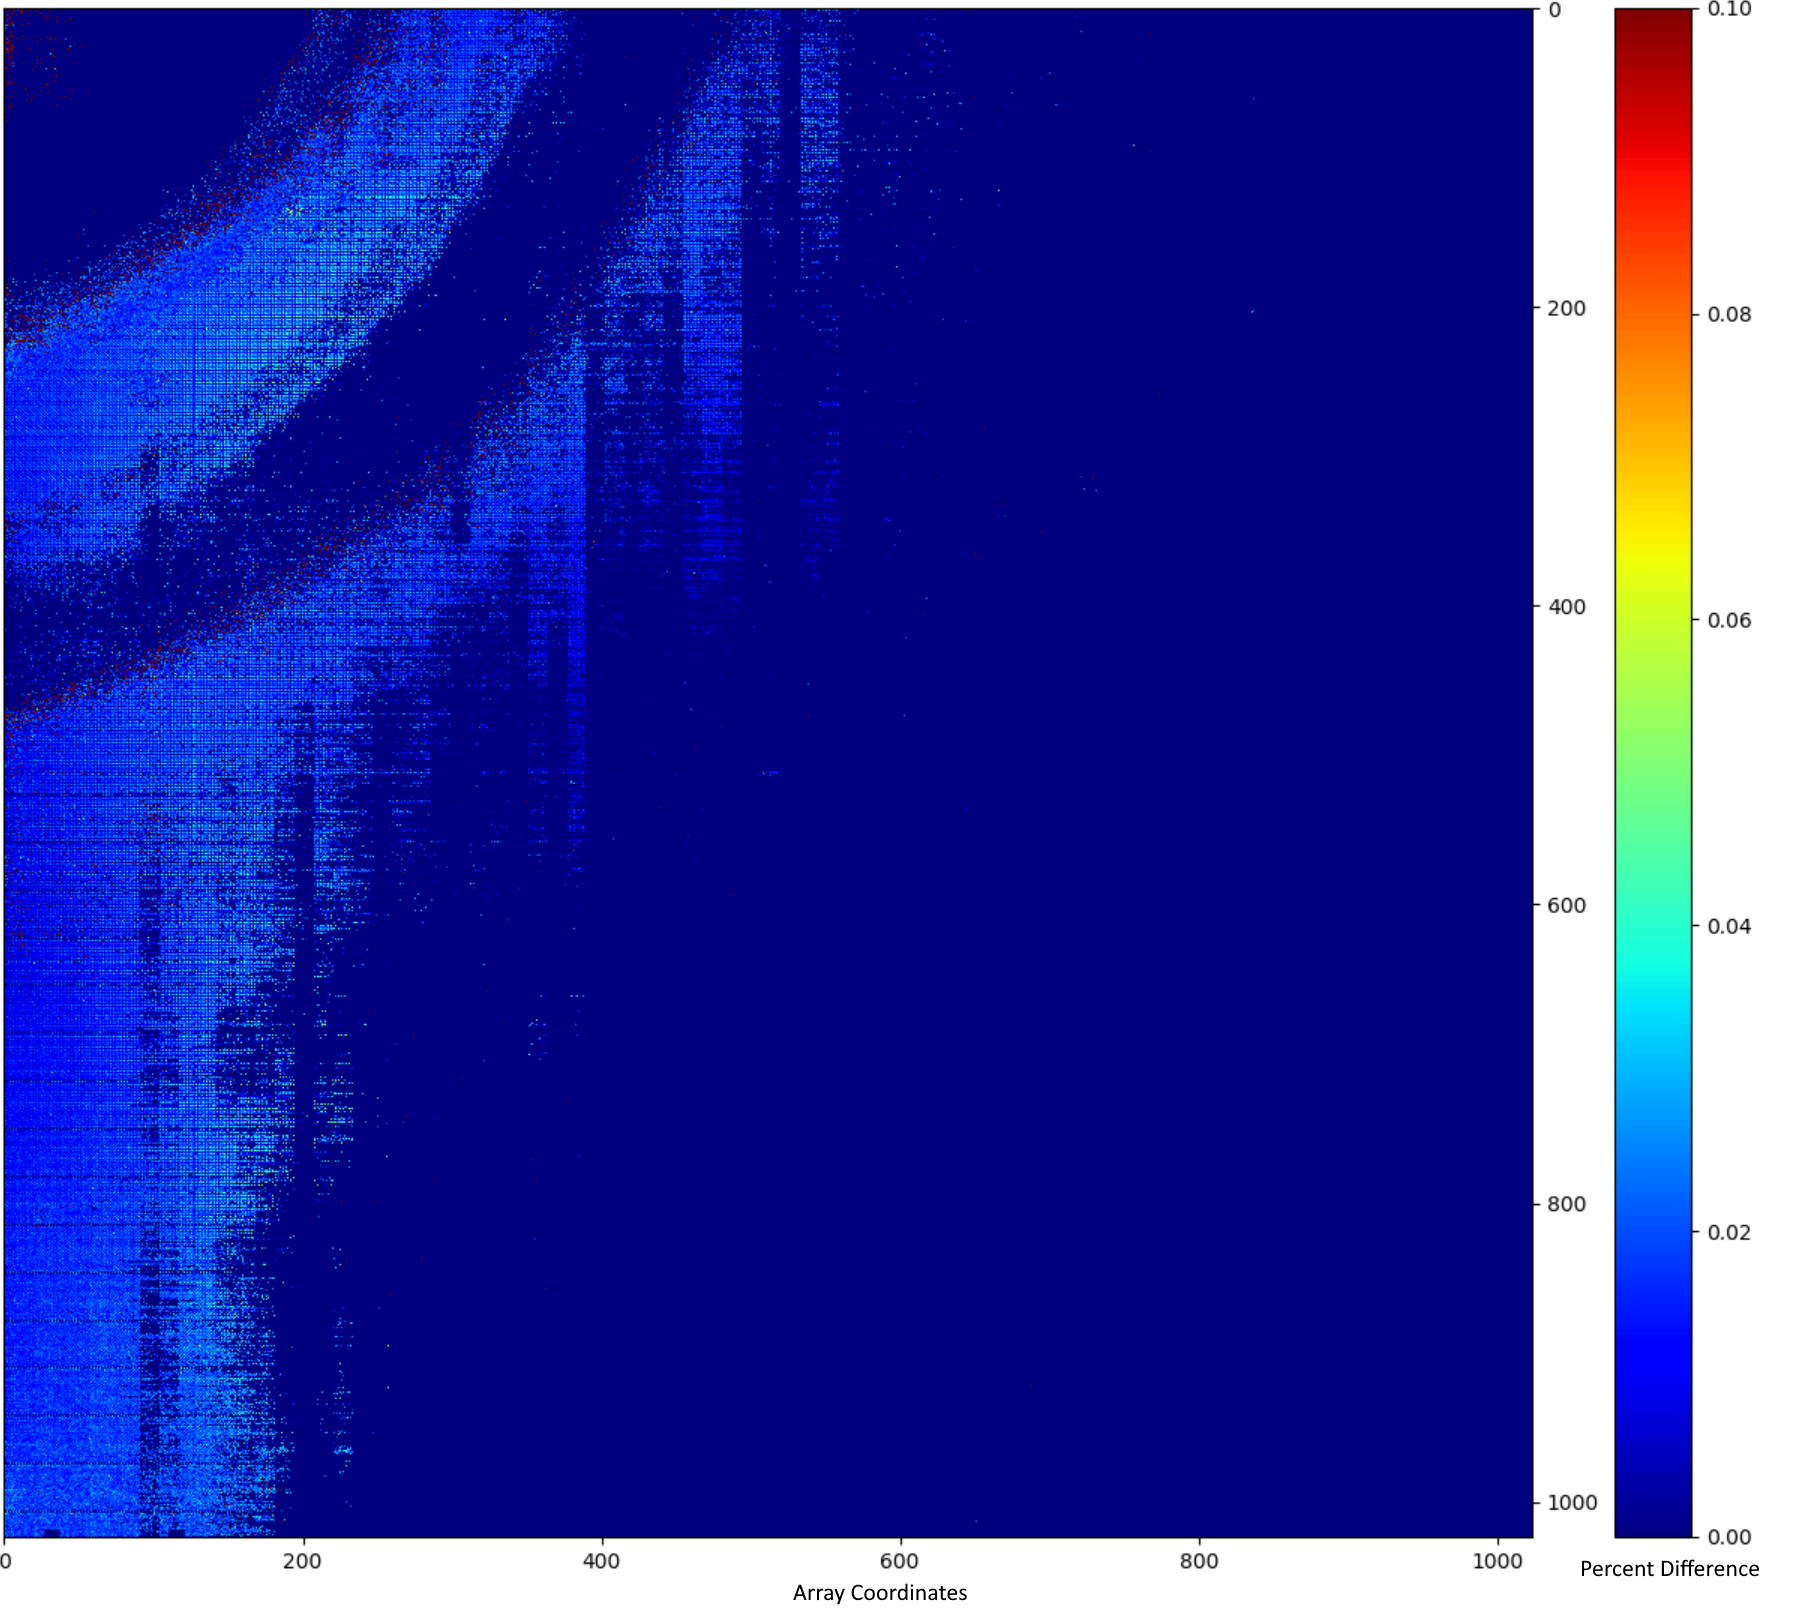
\includegraphics[width=1.0\textwidth]{fig/fractional_difference_snap.jpg}
                \caption{Fractional Difference Map of SNAP Firmware Output}
                \label{fig:fractional_difference_snap}
            \end{figure}

            The average variance for both the SNAP and PDP firmware is less than 4 percent. However, the PDP firmware has less variance in per pixel light output per run as indicated by the darker blue colors in the working portions of the array compared to the SNAP firmware. This is likely due to the static \mbox{200 megahertz} system clock used for driving an arrays pixels combined with the two flip-flop synchronization strategy utilized within the PDP firmware that is discussed in Chapter~\ref{sec:memorysync}. The earlier SNAP firmware used an HDMI clock signaling based approach to time triggering of events on the system side. Given that the clock is an input from an external HDMI card, it most likely has some noise. Another factor that may contribute to the larger variance is the fact that most functionality within SNAP used only the first HDMI card clock and ignored the second HDMI card clock. The crystal oscillators used for generating clock signals within devices typically have a finite precision due to various contributing factors such as thermal noise, power supply variations, and aging~\cite{Naval2002}. This means that oscillators within different physical devices may vary resulting in clock skew. Any inherit skew in oscillation could be further compounded by the fact that each HDMI card's data lines travel physically different trace paths to arrive within the FPGA. The PDP firmware on the other hand, makes no assumptions about input clock skew. The Memory synchronizer utilized within explicitly synchronizes the data of each HDMI card separately across clock domains to the system clock domain. Then it explicitly pulls data from each synchronized circular buffer independently. Overall, the behavioral results are promising for the PDP firmware.

        \subsubsection{Non-uniformity Corrected Imagery}
            Figure~\ref{fig:pdp_bird} shows an example of non-uniformity corrected IR imagery generated using the PDP firmware on an NSLEDS array. This particular array has much better yield than the one used for some of the earlier results presented in this chapter and is capable of displaying full images at a 1024 by 1024 resolution.

            \begin{figure}[t]
                \centering
                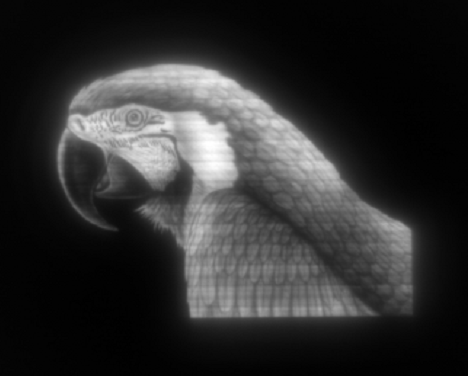
\includegraphics{fig/pdp_bird.png}
                \caption{Still Image Capture of a Non-uniformity Corrected Image from the PDP Firmware Operating at 100Hz}
                \label{fig:pdp_bird}
            \end{figure}

            Figure~\ref{fig:pdp_grid} shows a grid being displayed on the same array. The lower right-hand corner of the array has physical defects, but the majority of the array operates correctly. Interspersed in between the working pixels are a couple of dead pixels here and there. These look worse in a static grid map than in practice, as the brightness of neighboring pixels effectively hides individually defective pixels within an array. This is true as long as multiple pixels within a small region of an array are not defective as well. This is why Figure~\ref{fig:pdp_bird} shows no obvious dead pixels even though individual pixels are defective within the region that the image is displayed on.

            \begin{figure}[t]
                \centering
                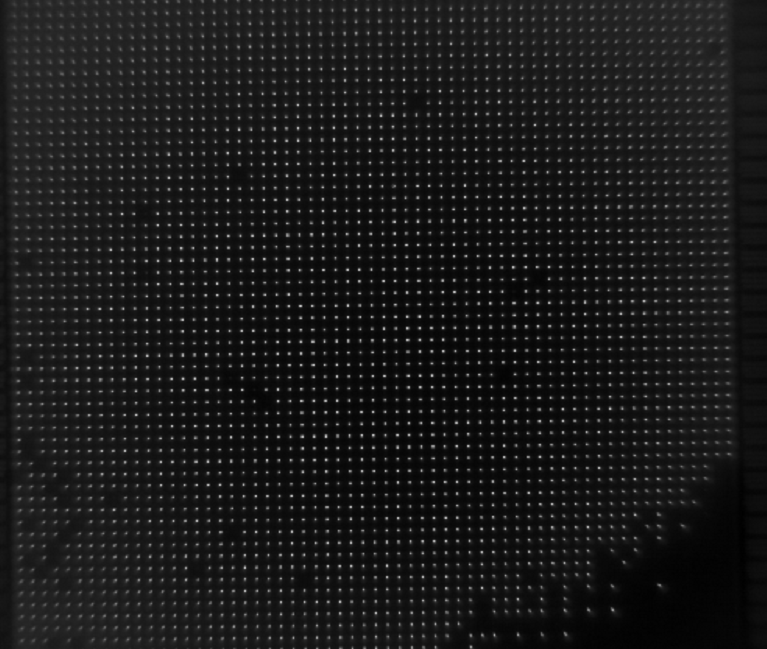
\includegraphics[width=0.76\textwidth]{fig/pdp_grid.png}
                \caption{Still Image Capture of a Grid from the PDP Firmware Operating at 100Hz}
                \label{fig:pdp_grid}
            \end{figure}

        \subsubsection{Analog Bandwidth}
            \label{sec:analog_bandwidth}
            Figure~\ref{fig:pdp_bird_comparison} shows the same IR image drawn at two different frame rates using the PDP firmware operating in backwards compatibility mode. In this mode, normal HDMI data is sent to an array at full resolution. At \mbox{100 hertz} operation, the image quality is much more uniform across pixels despite having low dynamic range when not non-uniformity corrected. At \mbox{400 hertz} operation, there are distinct banding patterns that are not visible at lower frame rates. These banding patterns are the result of limited analog bandwidth due to the time it takes for the analog portions of the system to settle which includes DAC settling time, amplifier settling time, RIIC internal timings, and emitter charge time. Under normal HDMI operation, it is difficult to correct for these issues at high-speed without introducing complicated compensation schemes such as analog or digital pre-emphasis filtering\footnote{Analog and digital pre-emphasis is used in many types of applications~\cite{BuckwalterEtAl2006, RafiqueEtAl2015, HuEtAl2017, ThaiEtAl2018, ZhouEtAl2020}.}.

            \begin{figure}[t]
                \centering
                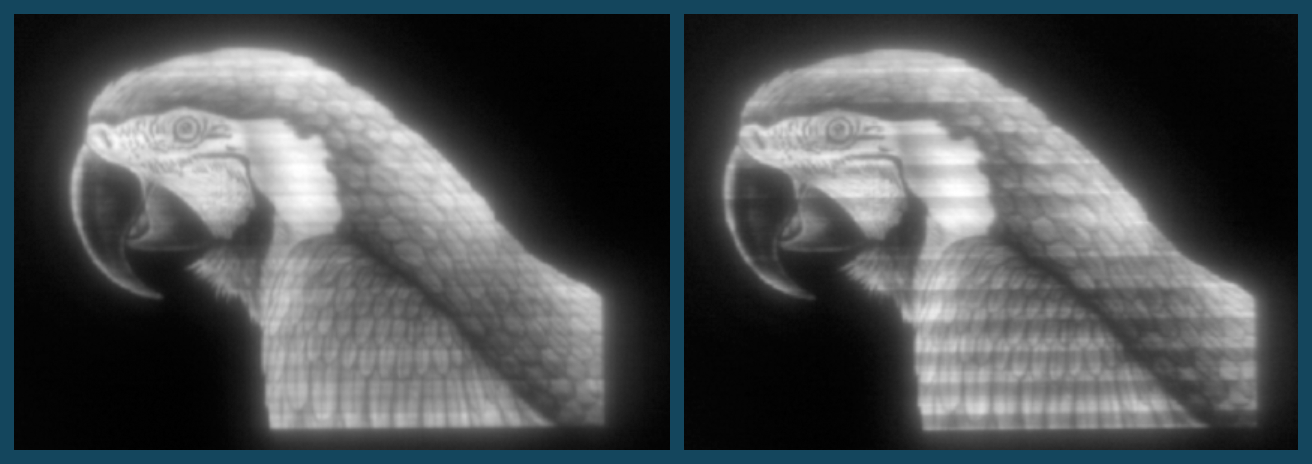
\includegraphics[width=1.0\textwidth]{fig/pdp_bird_comparison.png}
                \caption{Comparison of Imagery Captured from the PDP Firmware Operating at 100hz and 400hz}
                \label{fig:pdp_bird_comparison}
            \end{figure}

            Utilizing a packetized approach to display can help mitigate issues with high-speed display by providing more time for changing regions of a display to settle. Consider a 1024 by 1024 display operating at high speed. When packetized operation is utilized, ideally only subregions of the display are updated at high-speed and the portions of the array operating at low-speed are addressed at much slower rate; and thus, use much less analog bandwidth. The exact amount of analog bandwidth saved would depend on how much of the imagery needs to run at high-speed; however, this could be on the order of a 75 percent reduction in cases of low-speed backgrounds with small high-speed objects. This means that portions updating at high speed can be driven for longer amounts of times to allow for complete settling.
\section{Packetized Operation}
        This section shows various examples of the PDP firmware running at low-speed and high-speed operation to demonstrate the capabilities and versatility of a packetized display protocol. Additionally, multiple frame rate operation is demonstrated at high-speeds to show the capabilities of packetized operation.

    \subsection{Normal-speed}
        Figure~\ref{fig:low_speed_numbers} shows a series of counting numbers operating at low speeds. These were part of some of the initial demos used for testing packetized operation. This demo, in particular, ran at a number of different rates ranging from \mbox{60 hertz} to \mbox{240 hertz} operation. It was used as an initial verification of the firmware's packetized mode of operation.

        \begin{figure}[t]
            \centering
            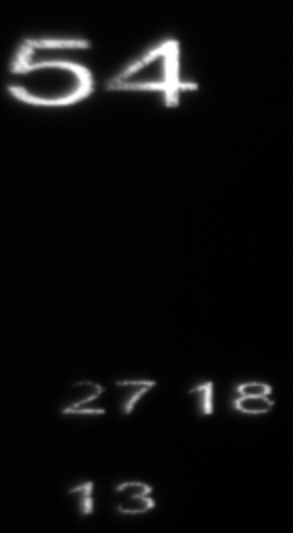
\includegraphics[width=0.15\textwidth]{fig/low_speed_numbers.png}
            \caption{Still Image Capture of Counting Numbers from the PDP Firmware Operating at 60Hz}
            \label{fig:low_speed_numbers}
        \end{figure}

        Other imagery included moving objects across the array at low-speed and moving changing numbers. Of particular interest was analyzing the boundaries of each packet for artifacts in overlapping packet regions and verifying that moving objects were not exhibiting partial display of previous packet data as these behaviors may indicate incorrect firmware operation. In initial testing, some implementation challenges included ensuring that the correct packet data was being sent from the driving computer to the CSE and verifying that the correct pixels were being addressed from within the firmware. The former was addressed by attaching the HDMI output links to loop-back capture devices and meticulously analyzing the output to ensure both the data ordering described in Chapter~\ref{sec:data_ordering} was being abided by, and that packet headers were being correctly specified. The latter was addressed by using an oscilloscope to analyze the address lines routed directly to the array.

    \subsection{High-speed}
        There have been a number of different high-speed demos used to test the PDP firmware at rates above \mbox{250 hertz} operation on an NSLEDS array. Due to the limitations in IR Camera speed, these were obtained by windowing the camera resolution down to allow for faster capture. Under full resolution, the IR cameras used can only reach \mbox{565 hertz} or \mbox{132 hertz} depending on the exact model.

        Figure~\ref{fig:high_speed_object} shows a still image for a demo of an object that moves along both the x and y dimensions of the array at \mbox{1 kilohertz}. When an edge is reached, the object bounces similar to the electronic game of Pong\cite{Alcorn1972}. This object was drawn using multiple PDP draw region packets embedded into a larger HDMI frame. For every packet, the {\it x start} and {\it y start} locations were modified. Drawing at this rate with normal full frame HDMI is impossible. At best, \mbox{240 hertz} may be used with sacrifices in image fidelity due to limited analog bandwidth as discussed in Chapter~\ref{sec:analog_bandwidth}.

        \begin{figure}[t]
            \centering
            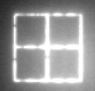
\includegraphics[width=0.15\textwidth]{fig/high_speed_object.png}
            \caption{Still Image Capture of a Moving Object from the PDP Firmware Operating at 1Khz}
            \label{fig:high_speed_object}
        \end{figure}

        Figure~\ref{fig:high_speed_numbers} shows a series of images for a number counting demo running at {2 kilohertz} operation. This demo consisted of both a static configuration in which a predefined location was used to display the number and a moving configuration in which the number would move around the array in both the x and y dimensions. In both configurations, the number would increment by one at the given frame rate. The object itself was drawn using individual PDP packets for each numerical digit. As with the previous example, drawing at this rate with normal full frame HDMI is impossible which demonstrates that packetized operation can achieve rates well beyond normal HDMI with the same hardware.

        \begin{figure}[t]
            \centering
            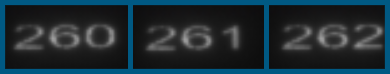
\includegraphics[width=0.7\textwidth]{fig/high_speed_numbers.png}
            \caption{Still Image Captures of a Counting Number from the PDP Firmware Operating at 2Khz}
            \label{fig:high_speed_numbers}
        \end{figure}

        Figure~\ref{fig:high_speed_rotating_object} shows a series of frames for a non-uniformity corrected rotating three-dimensional object running at {2 Kilohertz} operation. The object itself was drawn using individual PDP packets for each rotation. Notably, even with the limited resolution of the IR camera when operating at a high-speed, the object is clear and distinct during each rotation. This demonstrates that packetized operation can indeed mitigate analog performance issues as discussed in Chapter~\ref{sec:analog_bandwidth}. A small object such as this could be displayed with a slow-speed background without sacrificing image quality which is representative of some types of IR imagery used in practice.

        \begin{figure}[t]
            \centering
            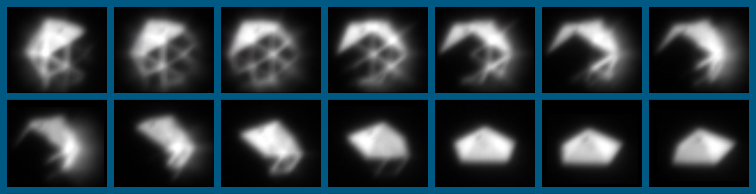
\includegraphics[width=0.7\textwidth]{fig/high_speed_rotating_object.png}
            \caption{Still Images Captures of a Non-uniformity Corrected Rotating Object from the PDP Firmware Operating at 2Khz}
            \label{fig:high_speed_rotating_object}
        \end{figure}

    \subsection{Multi-frame Rate}
        Figure~\ref{fig:pdp_multi_frame_rate} shows a series of frames for a multi-frame rate display of numbers using the PDP firmware. The small bright number was updated at \mbox{800 hertz}, the small background numbers was updated at \mbox{100 hertz}, and the large number was updated at \mbox{2 hertz}. Each number was drawn using individual PDP region packets. Similar to other demos discussed in this chapter, each number was incremented at the corresponding frame rate. This demonstrates that multiple framerate display operates correctly within the firmware and is able to achieve rates much higher than possible with the same hardware utilizing conventional display technology.

        \begin{figure}[t]
            \centering
            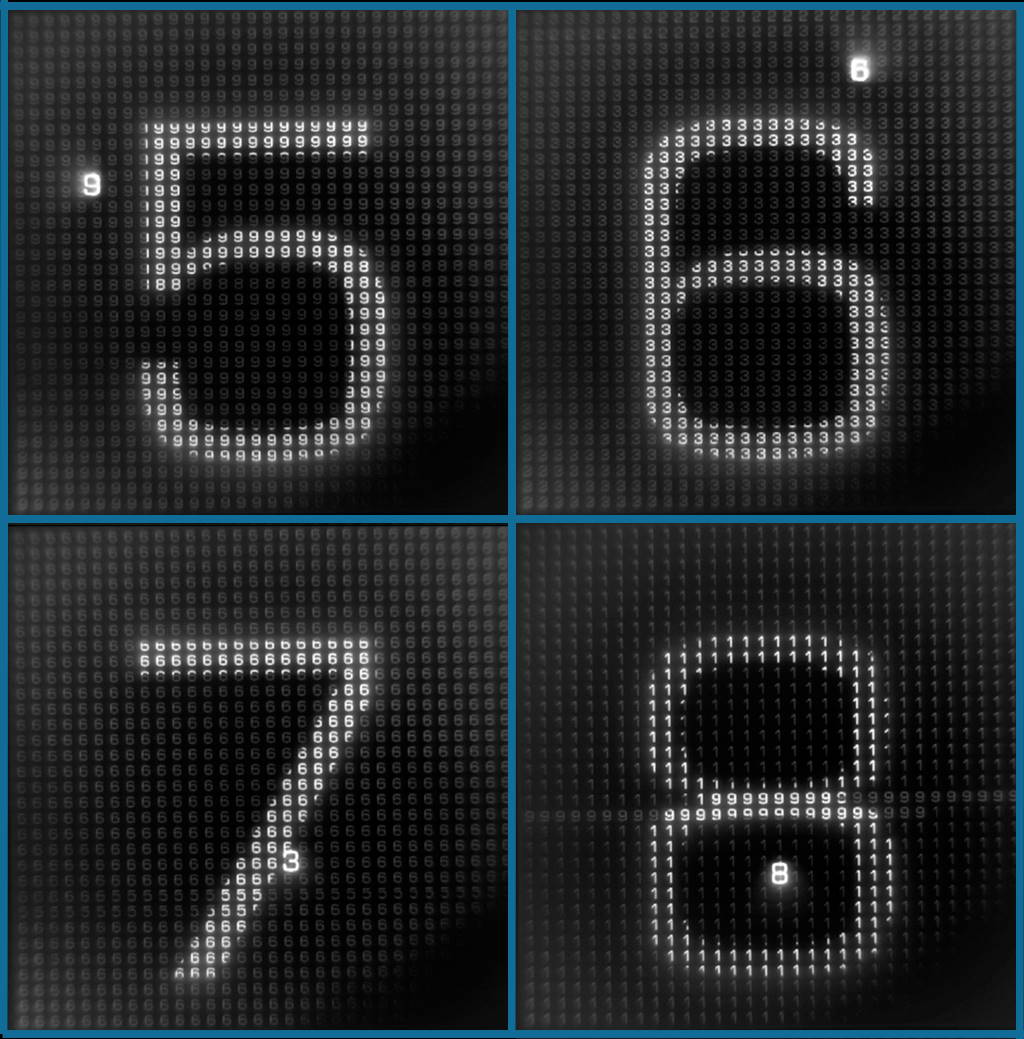
\includegraphics[width=0.80\textwidth]{fig/pdp_multi_frame_rate.jpg}
            \caption{Still Image Captures of a Bouncing Number, Small Background Numbers, and a Large Number from the PDP Firmware Operating at 800Hz, 100Hz, and 2Hz, Respectively}
            \label{fig:pdp_multi_frame_rate}
        \end{figure}

\section{Summary}
    The experimental results provided within this chapter make a strong argument to the benefit of packetized display technology for use in future high-speed IRSP systems. A wide breadth of different experiments was shown including normal backwards compatible HDMI operation, low-speed packetized display, high-speed packetized display, and high-speed multiple frame rate operation.

    Taken together, these demonstrate that packetized operation is capable of vastly improving performance in bandwidth starved environments. The improvements in digital bandwidth utilization show that substantially higher frame rates can be achieved. Additionally, multiple frame rate operation, in particular, enables better analog performance by allowing analog bandwidth to be to be reserved for high-speed updates of pixel regions which in turn yields improved overall image quality. In contrast, conventional display technology requires that analog bandwidth be apportioned equally for all pixels which results in considerably inferior image quality at high-speeds.

    The subsequent and final chapter of this dissertation is devoted to an overall discussion of the journey through the architectural development and implementation of a Packetized Display Protocol (PDP) architecture for Infrared Scene Projection Systems (IRSPs).
